\documentclass[12pt,a4paper]{article}
\usepackage[UTF8]{ctex}
\usepackage{graphicx}
\usepackage[margin=1cm]{geometry}
\usepackage{hyperref}

% 去除页眉页脚
\pagestyle{empty}

% 标题设置
\title{\textbf{\Huge Social-RAG 论文思维导图}\\[1em]
\Large 从群体交互中检索以实现 AI 生成的社会化基础\\[0.5em]
\normalsize (CHI 2025)}
\author{\large 人机交互课程作业}
\date{\today}

\begin{document}

\maketitle
\thispagestyle{empty}

\newpage

% 英文版思维导图 - 整页显示
\begin{figure}[p]
    \centering
    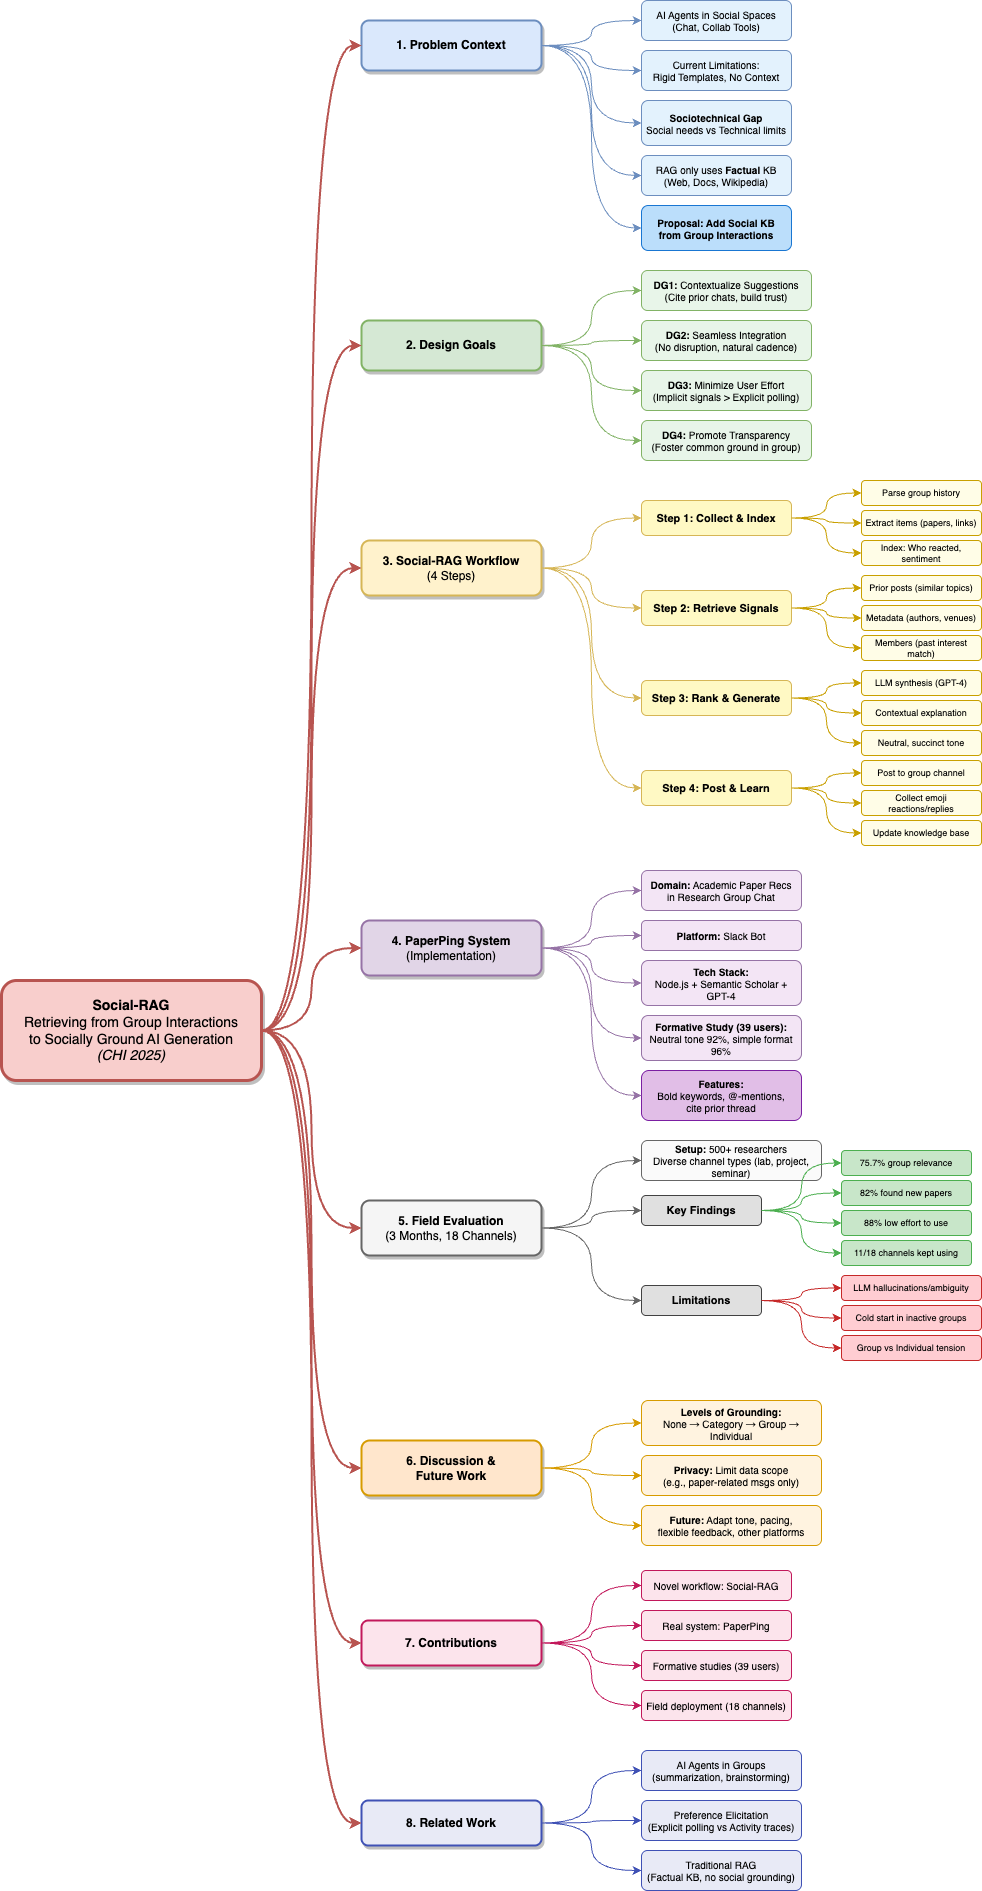
\includegraphics[width=\textwidth,height=\textheight,keepaspectratio]{Social_RAG_Mind_Map.png}
\end{figure}

\newpage

% 中文版思维导图 - 整页显示
\begin{figure}[p]
    \centering
    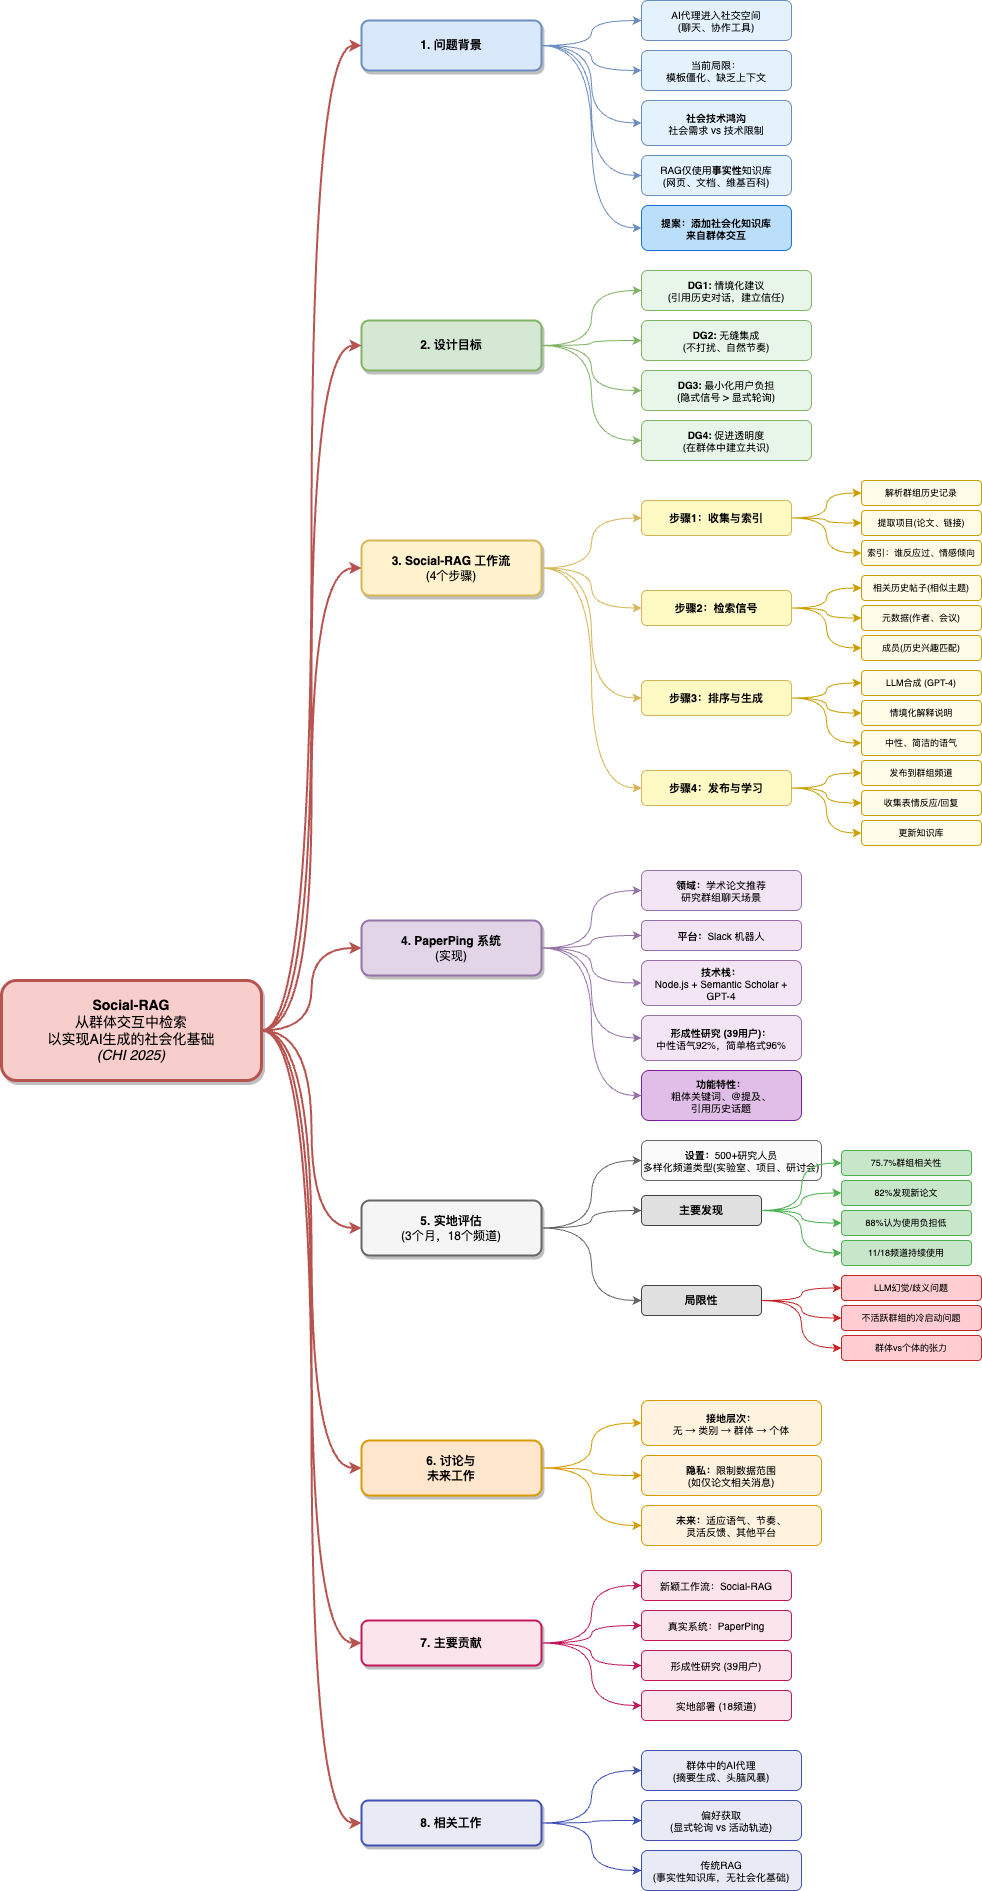
\includegraphics[width=\textwidth,height=\textheight,keepaspectratio]{Social_RAG_Mind_Map_CN.png}
\end{figure}

\end{document}
